\setcounter{figure}{0} % Compensate summary part one in 'part' counter 
%\addcontentsline{toc}{part}{Summary of Part I: Reinforcement Learning in Finite State and Action Spaces}
%\part{Summary of Part I: Reinforcement Learning in Finite State and Action Spaces}
\pdfbookmark[1]{Summary of Part I: Reinforcement Learning in Finite State and Action Spaces}{Sum_Part_One} 
\title[Summary of Part I]{Summary of Part I: Reinforcement Learning in Finite State and Action Spaces}  
\date{}  
\frame{\titlepage}
\renewcommand{\thefigure}{S-I.\arabic{figure}} 

%%%%%%%%%%%%%%%%%%%%%%%%%%%%%%%%%%%%%%%%%%%%%%%%%%%%%%%%%%%%%
%% Common Key Ideas to Explored RL Methods %%
%%%%%%%%%%%%%%%%%%%%%%%%%%%%%%%%%%%%%%%%%%%%%%%%%%%%%%%%%%%%%
\frame{\frametitle{Common Key Ideas to all Discussed RL Methods so far}
\begin{enumerate}
	\item Estimating and comparing value functions
	\item Backing up values along actual or possible state trajectories
	\item Usage of GPI mechanism to maintain an approximate value function and policy trying to improve each of them on the basis of the other
\end{enumerate}
\begin{figure}
	\subfloat{
		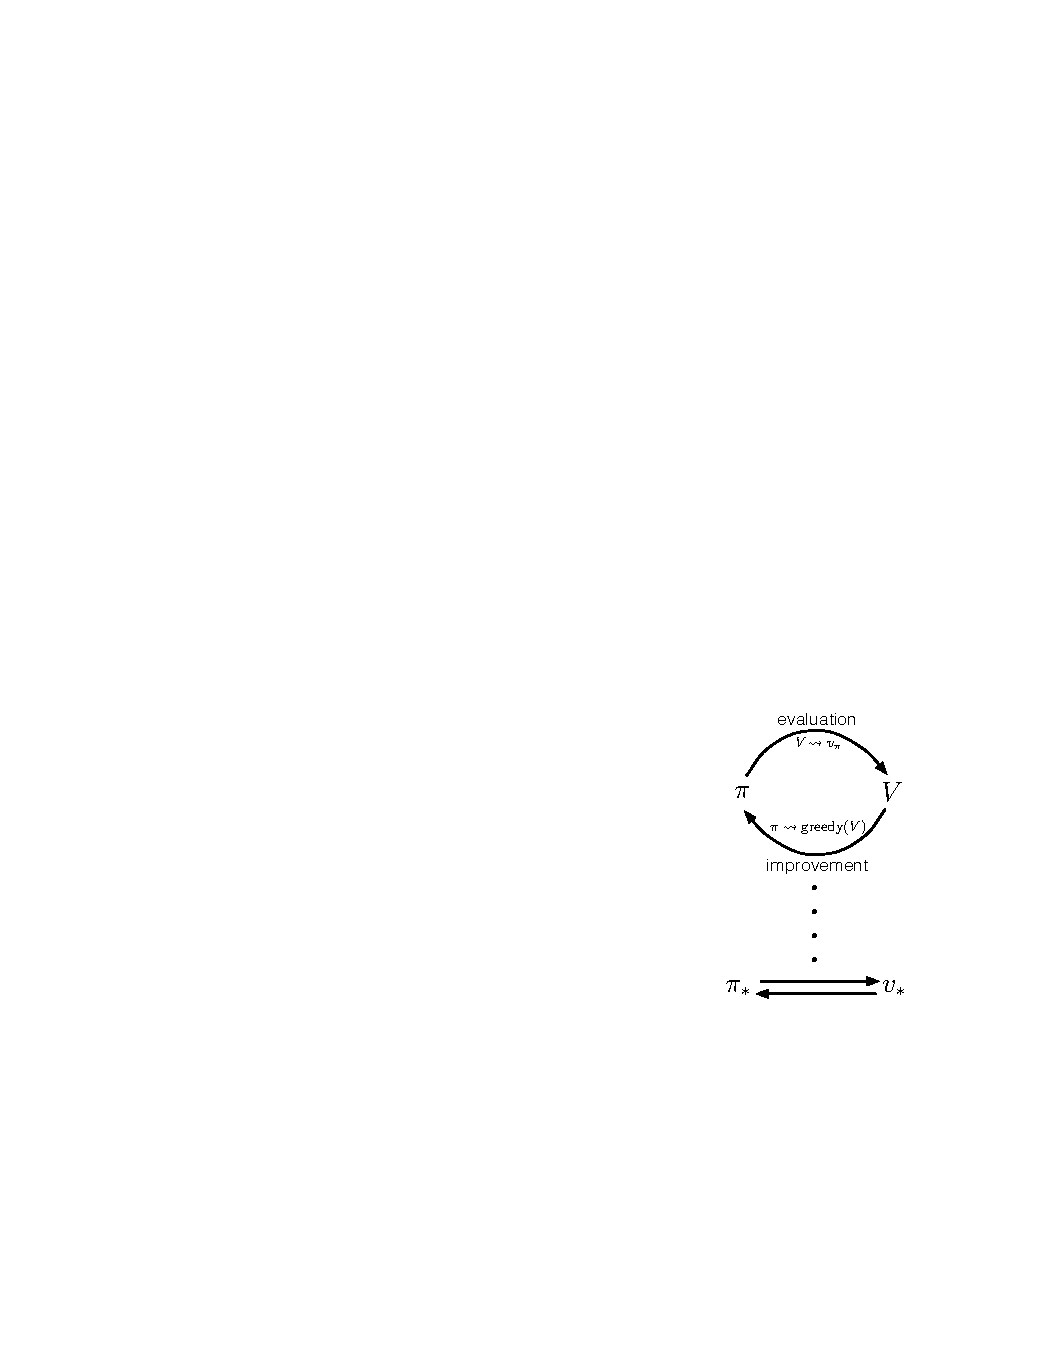
\includegraphics[height=4cm]{fig/lec03/GPI_01.pdf}
	}
	\hspace{1cm}
	\subfloat{
		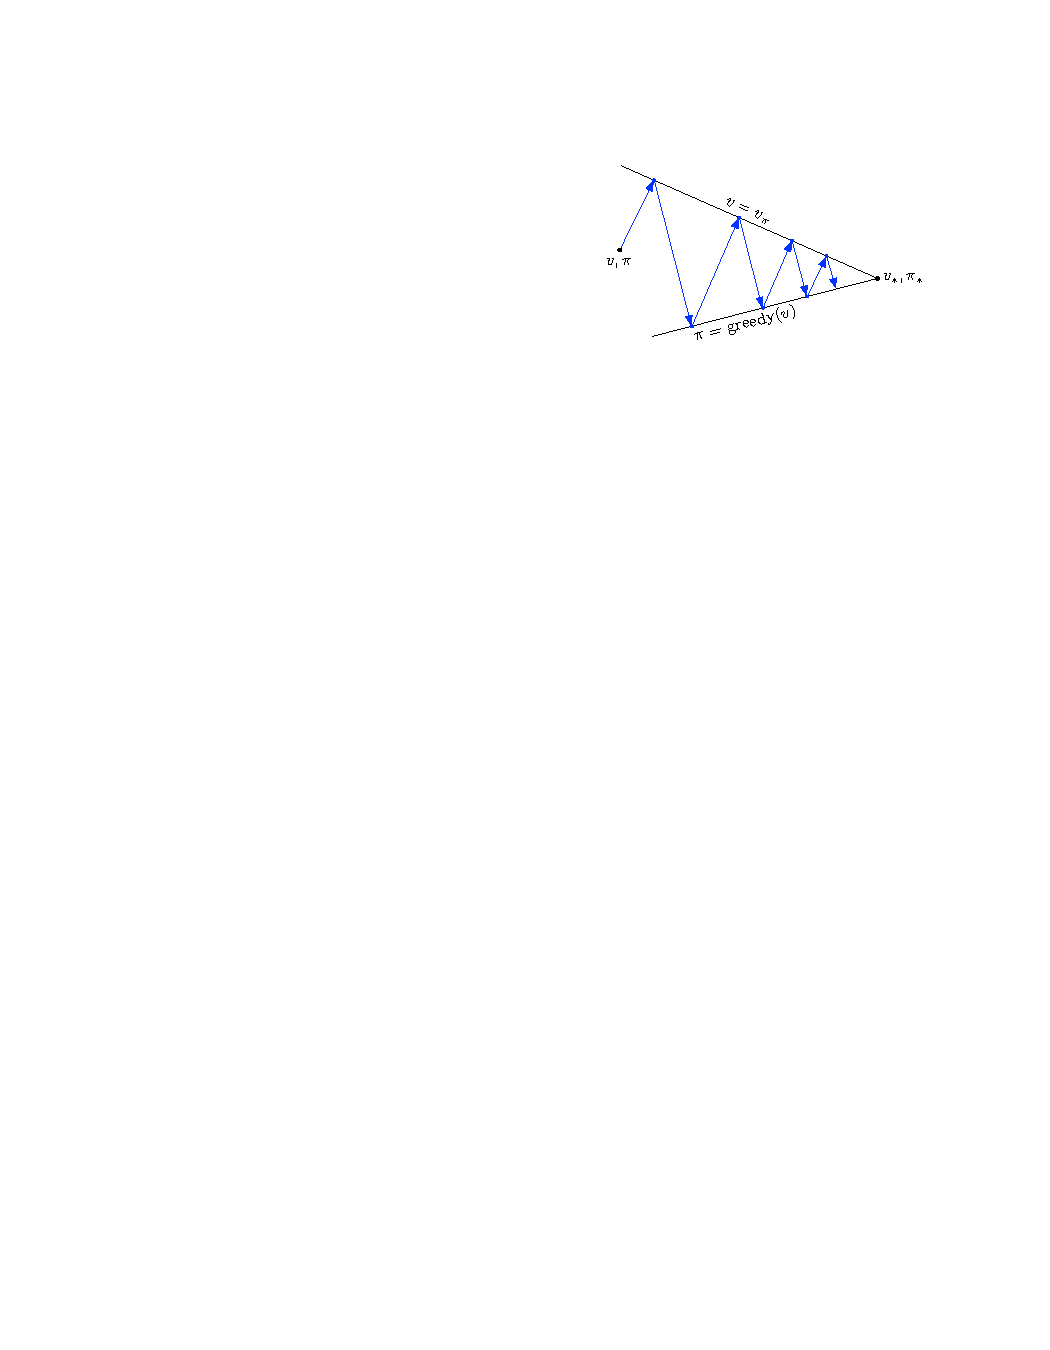
\includegraphics[height=4cm]{fig/lec03/GPI_02.pdf}
	}
\caption{Generalized policy iteration (GPI) as a mutual building block of all previously discussed RL methods (source: R. Sutton and G. Barto, Reinforcement learning: an introduction, 2018, \href{https://creativecommons.org/licenses/by-nc-nd/2.0/}{CC BY-NC-ND 2.0})}
\end{figure}
}


%%%%%%%%%%%%%%%%%%%%%%%%%%%%%%%%%%%%%%%%%%%%%%%%%%%%%%%%%%%%%
%% Two Important RL Dimensions: Depth and Width of Updates %%
%%%%%%%%%%%%%%%%%%%%%%%%%%%%%%%%%%%%%%%%%%%%%%%%%%%%%%%%%%%%%
\frame{\frametitle{Two Important RL Dimensions: Update Depth and Width}
\begin{figure}
	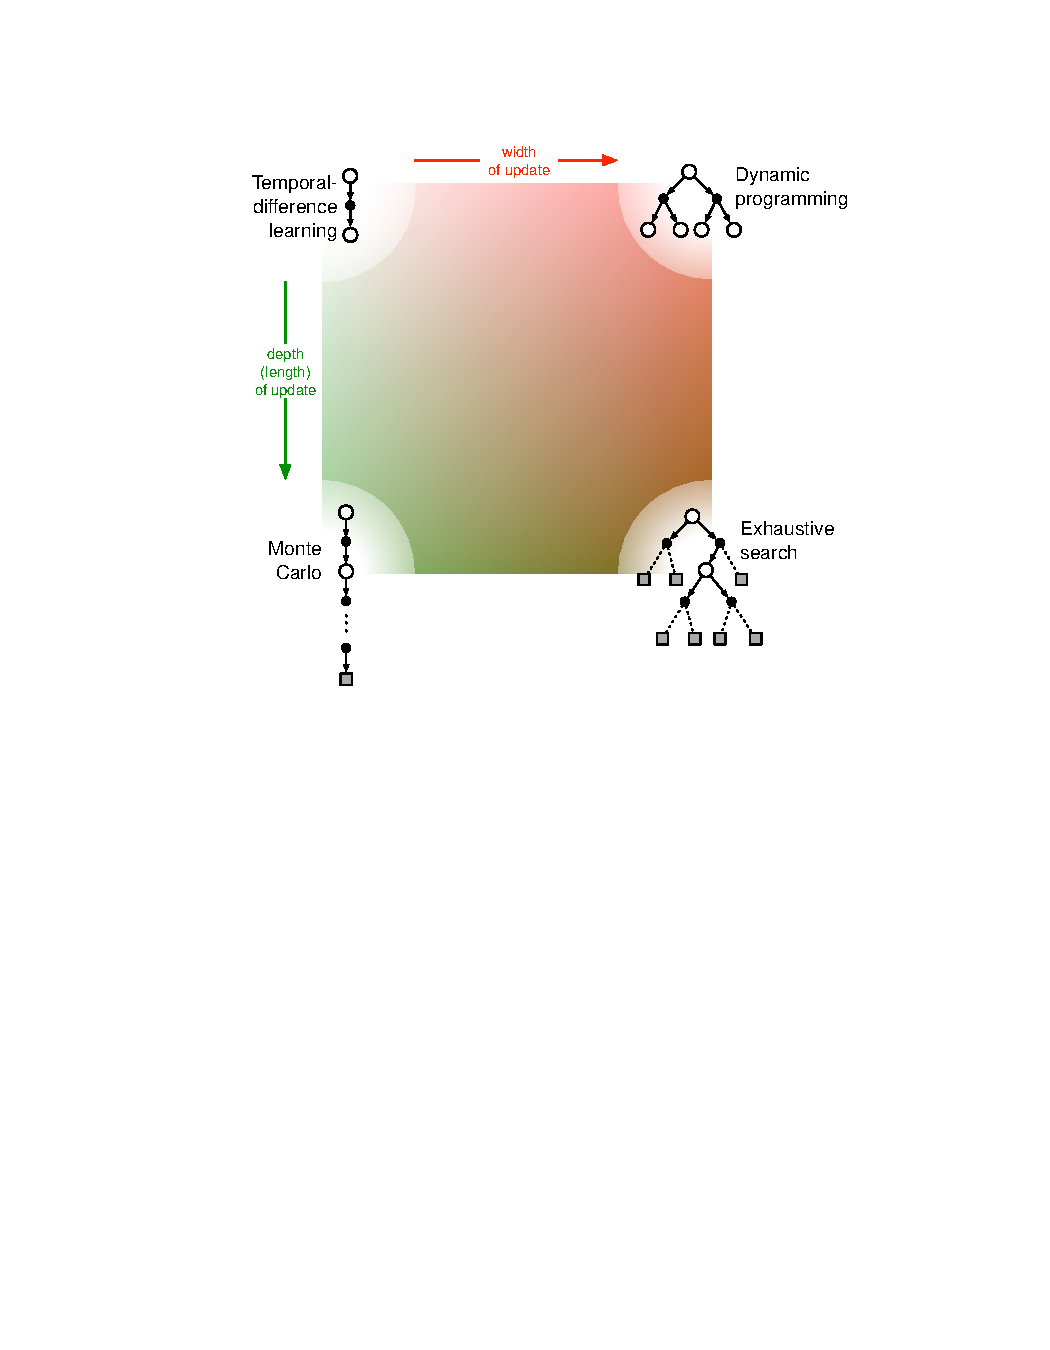
\includegraphics[width=7cm]{fig/lec06/Compare_RL_Methods_Update.pdf}
	\caption{A slice through the RL method space (source: R. Sutton and G. Barto, Reinforcement learning: an introduction, 2018, \href{https://creativecommons.org/licenses/by-nc-nd/2.0/}{CC BY-NC-ND 2.0})}
\end{figure}
}

%%%%%%%%%%%%%%%%%%%%%%%%%%%%%%%%%%%%%%%%%%%%%%%%%%%%%%%%%%%%%
%% Other Important RL Dimensions %%
%%%%%%%%%%%%%%%%%%%%%%%%%%%%%%%%%%%%%%%%%%%%%%%%%%%%%%%%%%%%%
\frame{\frametitle{Other Important RL Dimensions}
Selected, non-exhaustive list:
\begin{itemize}
	\item \hl{Problem space}: How many states and actions? Stochastic vs. deterministic environment? Stationary?\pause
	\item \hl{Policy objective}: on-policy vs. off-policy? Explicit vs. implicit policy?\pause
	\item \hl{Task}: Episodic vs. continuing?\pause
	\item \hl{Return definition}: Discounting? General reward design?\pause
	\item \hl{Value}: State vs. action value estimation? \pause
	\item \hl{Model}: Required? Distribution vs. sample models? Learning vs. a priori (expert) knowledge?\pause 
	\item \hl{Exploration}: How to search for new policies?\pause
	\item \hl{Update order}: synchronous vs. asynchronous? If latter, which order?\pause
	\item \hl{Experience}: simulated vs. real experience? Memory length and style?
	\item ...
\end{itemize}
}

%%%%%%%%%%%%%%%%%%%%%%%%%%%%%%%%%%%%%%%%%%%%%%%%%%%%%%%%%%%%%
%% Outlook %%
%%%%%%%%%%%%%%%%%%%%%%%%%%%%%%%%%%%%%%%%%%%%%%%%%%%%%%%%%%%%%
\frame{\frametitle{Outlook}
First part of the course:
\begin{block}{Reinforcement learning on small finite action and state spaces}
The problem space is such small that RL methods based on look-up tables are applicable.
\end{block}\pause
\vspace{0.5cm}
Second part of the course::
\begin{block}{Reinforcement learning using function approximators}
The problem space is either continuous or contains an unfeasible large amount of discrete state-action pairs. Value estimates, models or explicit policies stored in look-up tables would let the memory demand explode. Modifications and extensions of available RL algorithms using function approximators are required.    
\end{block}
}

%%%%%%%%%%%%%%%%%%%%%%%%%%%%%%%%%%%%%%%%%%%%%%%%%%%%%%%%%%%%%
%% Final Slide %%
%%%%%%%%%%%%%%%%%%%%%%%%%%%%%%%%%%%%%%%%%%%%%%%%%%%%%%%%%%%%%
\frame{\frametitle{The End for Today}
\vspace{-0.25cm}
\begin{figure}
\hspace*{-0.5cm}
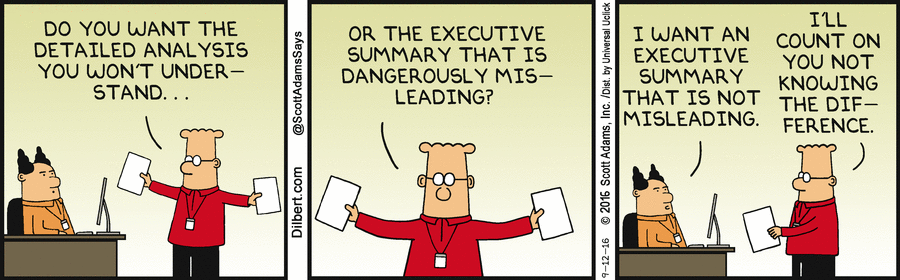
\includegraphics[width=10cm]{fig/lec07/dilbert2.png}
\end{figure}
\vspace{1cm}
\centering
Thanks for your attention and have a nice week!
}

\renewcommand{\thefigure}{\arabic{part}.\arabic{figure}}